\subsection{System modeling and design.}
Use UML to describe system context environment, objects, and key processes.

\textbf{System Bussiness Object}

According to the latest system requirement specifactions(SRS), 
the system will have the following bussiness objects(BO) which serve the MVC.

% http://bib-it.sourceforge.net/help/fieldsAndEntryTypes.php
Fig. \ref{fig:bo_classes_1} shows the very basic BOs of the system. 
\textbf{Record} will be the topmost general BO above any other BO.
\textbf{Researcher} will represent the solid system user.
\textbf{PaperMetadata} will represent paper informations.

\begin{figure*}[t]
	\centering
	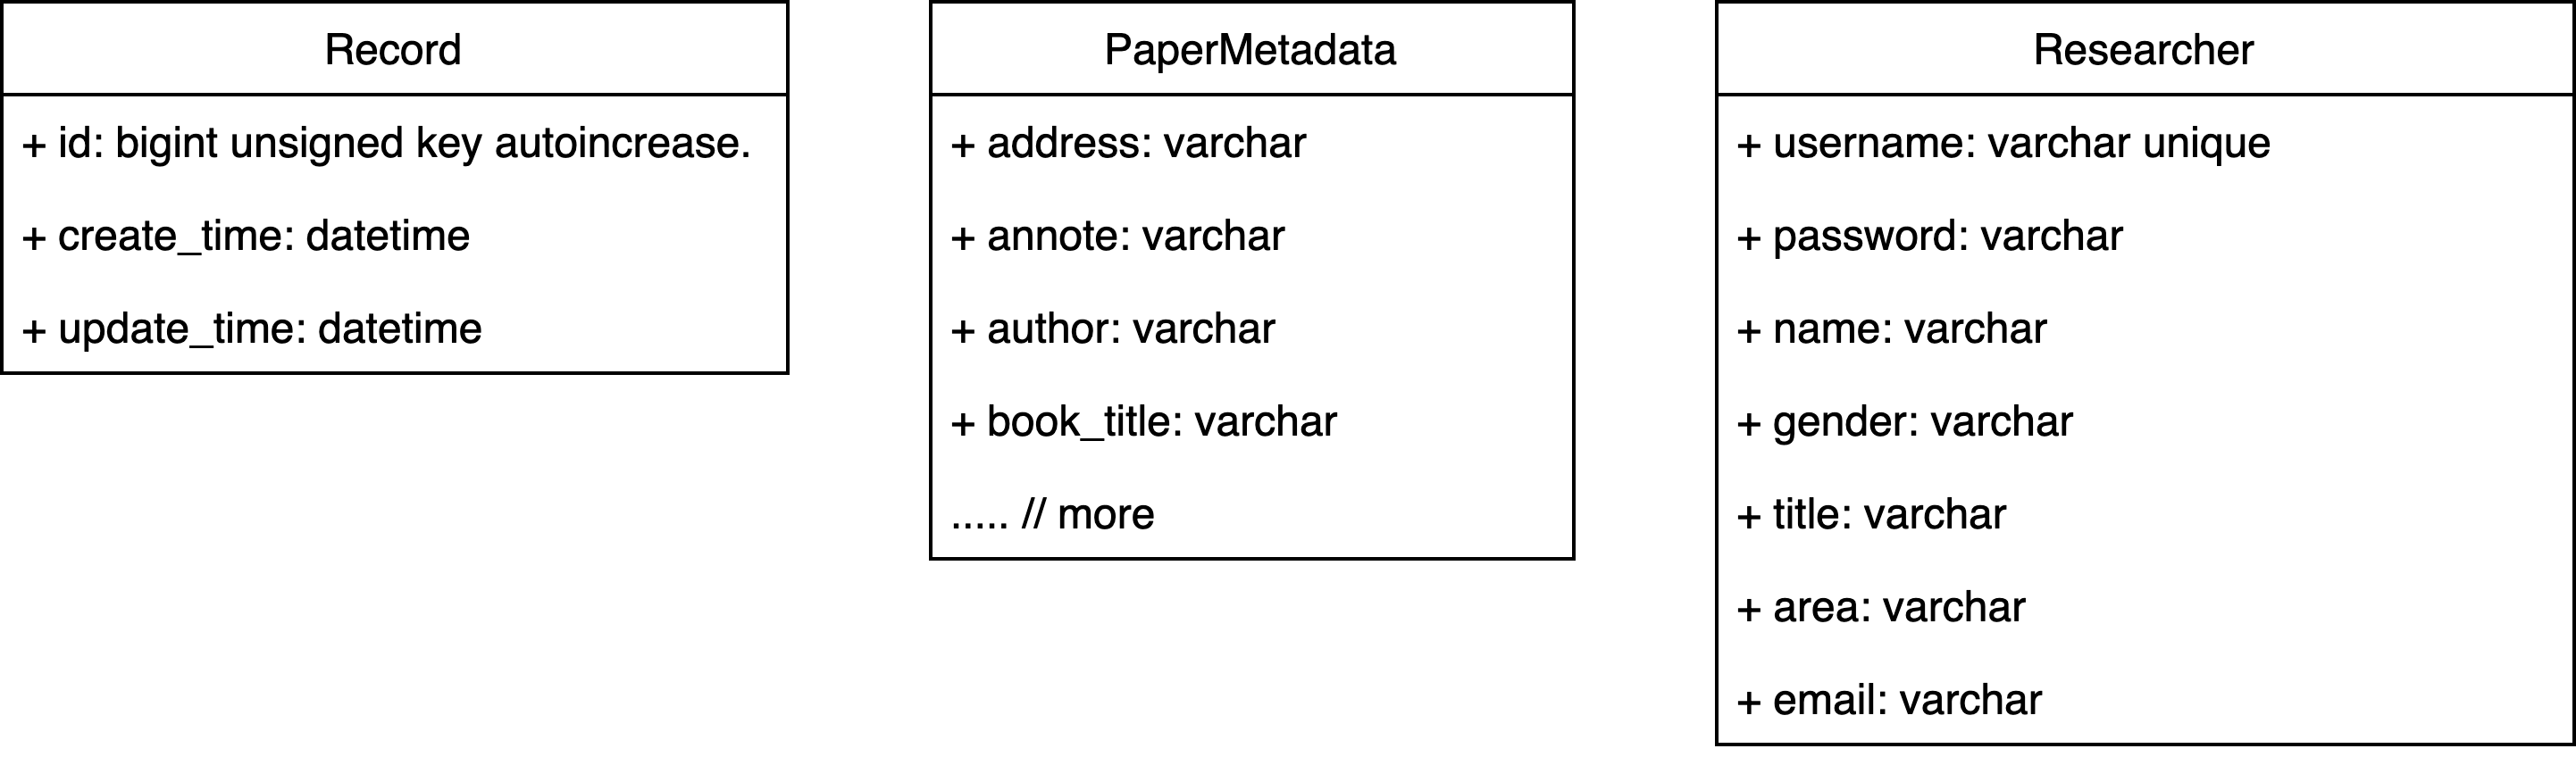
\includegraphics[width=\textwidth]{./img/bo_classes_1.png}
	\caption{Bussiness Objects Part1: Record, Researcher, PaperMetadata}
	
	\label{fig:bo_classes_1}
\end{figure*}


Fig. \ref{fig:bo_classes_2} shows the BOs which represent the users' preference about certain paper. 
\textbf{PaperComment} will be the comment wrote by the user.
\textbf{PaperLikeAndDislike} will represent the preference from the user.

\begin{figure*}[t]
	\centering
	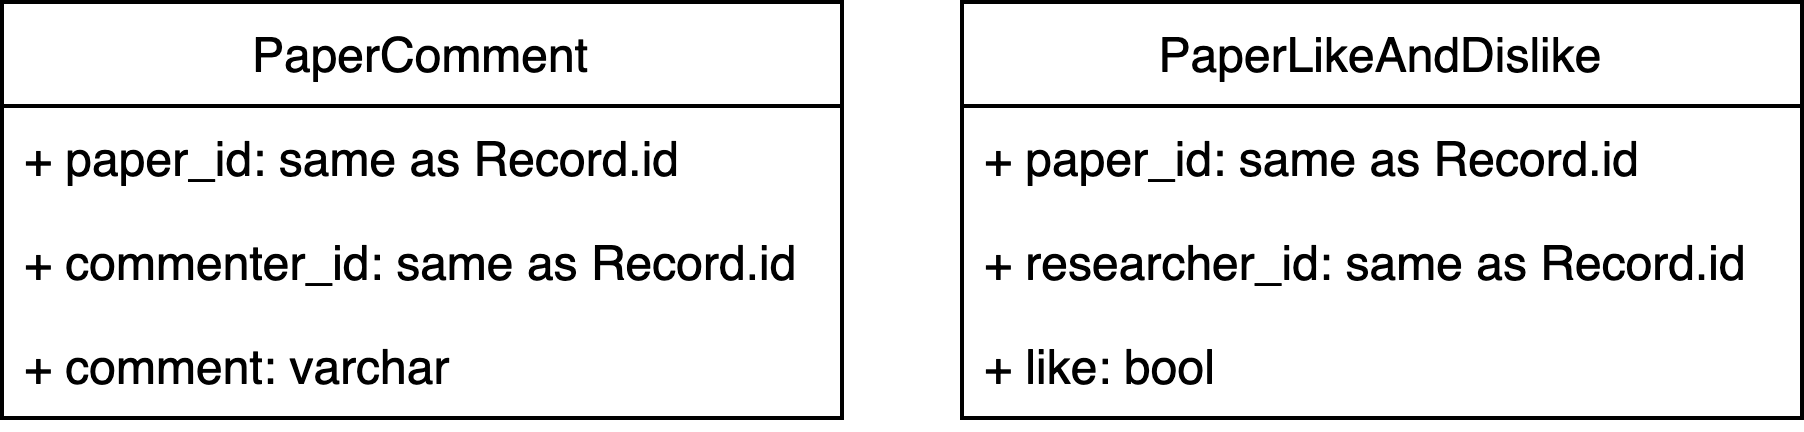
\includegraphics[width=0.7\textwidth]{./img/bo_classes_2.png}
	\caption{Bussiness Objects Part2: PaperComment, PaperLikeAndDislike}
	
	\label{fig:bo_classes_2}
\end{figure*}

Fig. \ref{fig:bo_classes_3} shows the BOs which represent the users' paper collection. 
\textbf{PaperCollectionCat} will be the collections which are created by the user.
\textbf{PaperCollectionRecord} will represent the single paper that collected within certain collection category.

\begin{figure*}[t]
	\centering
	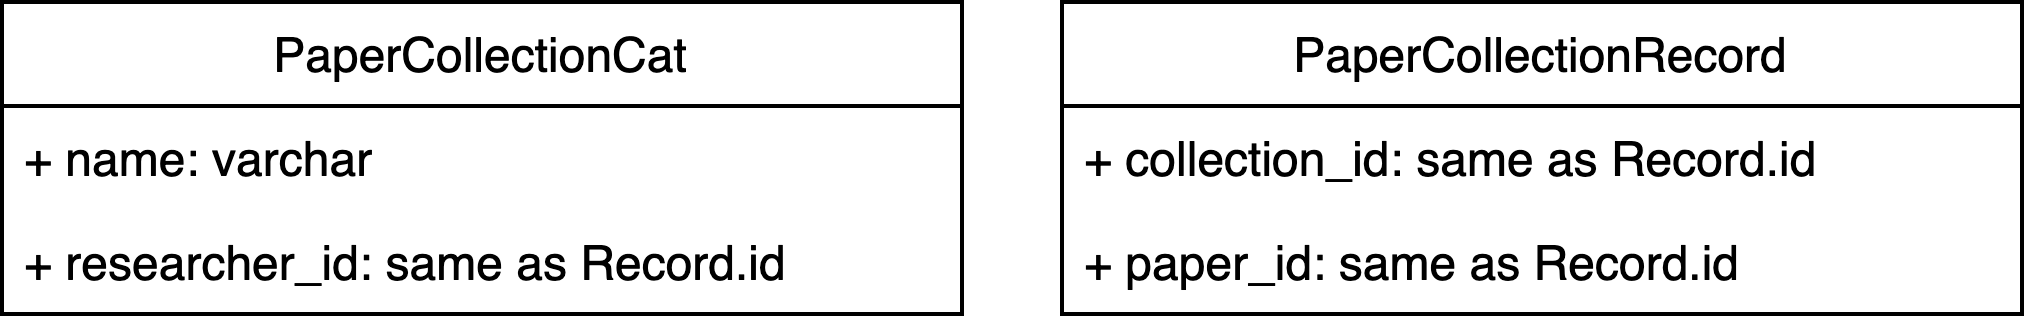
\includegraphics[width=0.7\textwidth]{./img/bo_classes_3.png}
	\caption{Bussiness Objects Part3: PaperCollectionCat, PaperCollectionRecord}
	
	\label{fig:bo_classes_3}
\end{figure*}

Fig. \ref{fig:bo_classes_4} shows the BOs which will gain the benefits from the ICDE. 
\textbf{UserOperationRecord} will be the records that are created by the system whenever the system user performs paper-relevant actions.
\textbf{PaperClickTrending} will represent the trending of how many clicks on certain papers, 
this data will generate by the system using the data recorded by ICDE.
\textbf{SearchTermTrending} will represent the trending of the hottest search terms.

\begin{figure*}[t]
	\centering
	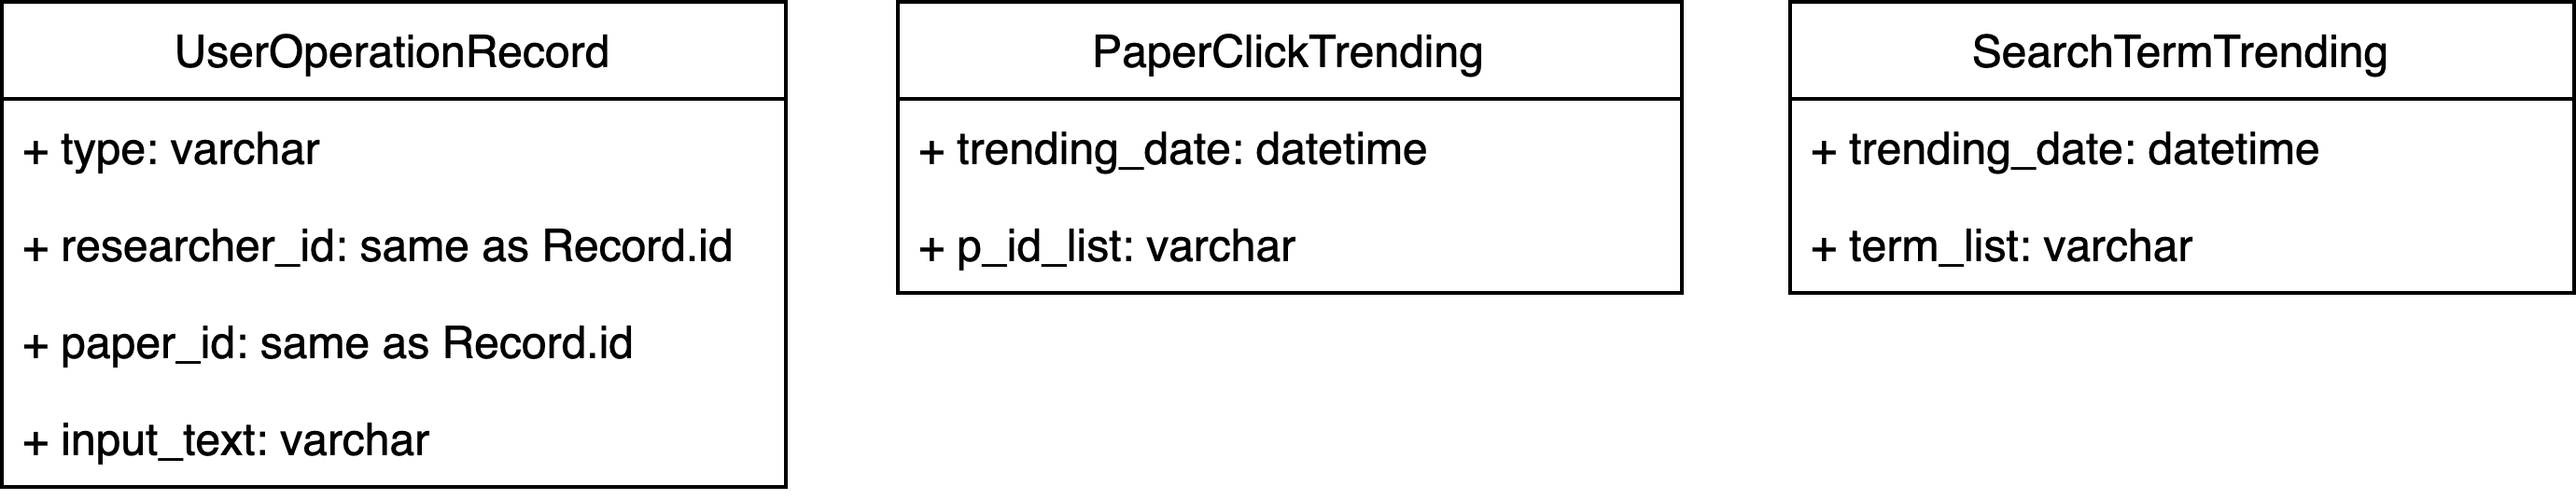
\includegraphics[width=0.85\textwidth]{./img/bo_classes_4.png}
	\caption{Bussiness Objects Part4: UserOperationRecord, PaperClickTrending, SearchTermTrending}
	
	\label{fig:bo_classes_4}
\end{figure*}


Fig. \ref{fig:bo_classes_5} shows the BOs which represent Team features of the system. 
\textbf{ResearchTeam} will represent a research team.
\textbf{ResearchTeamAuthRecord} will represent the relationship between users and teams.

\begin{figure*}[t]
	\centering
	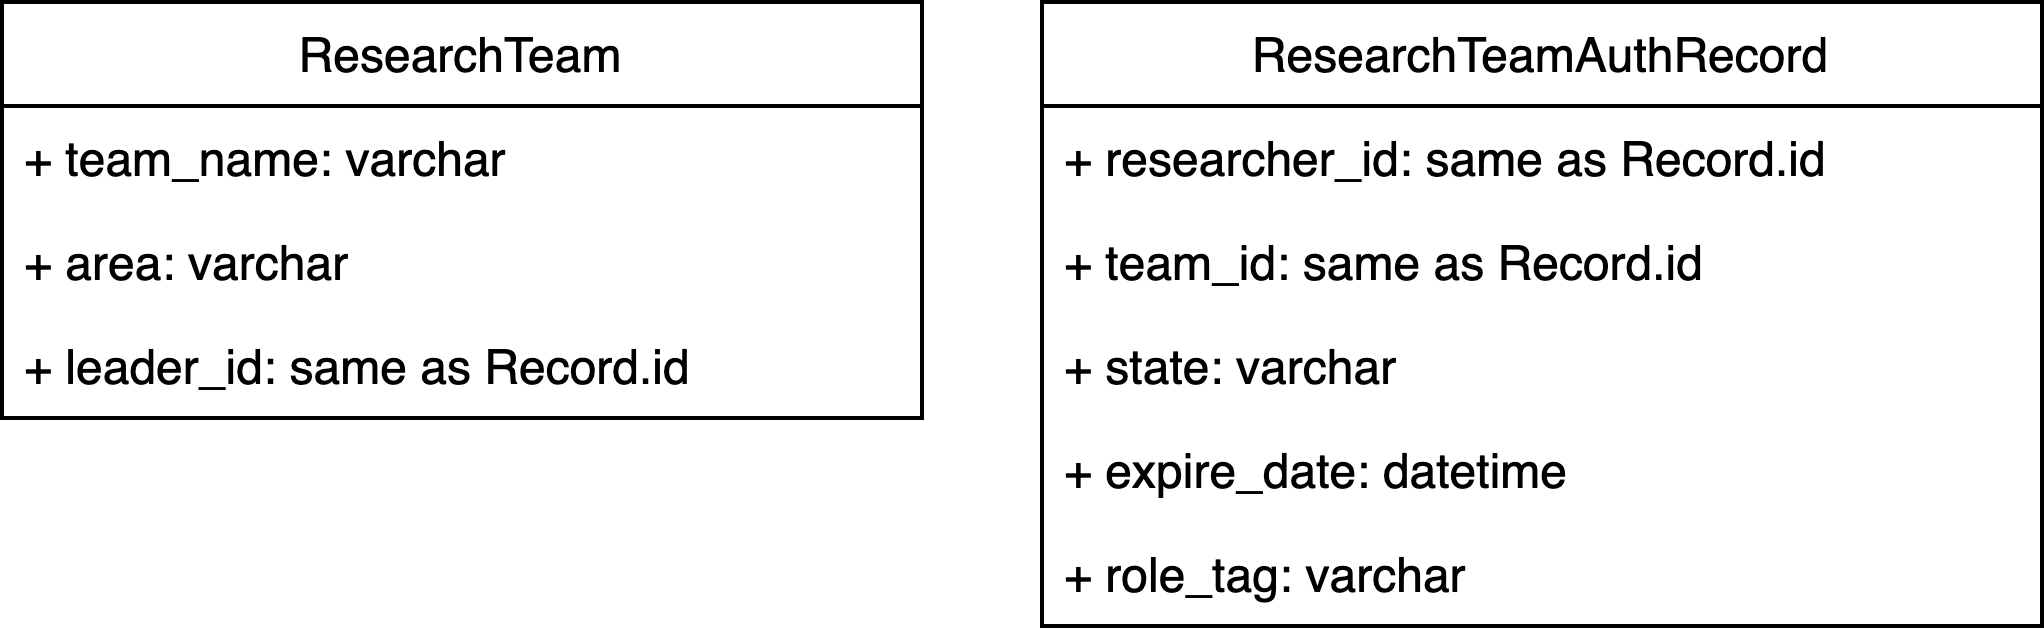
\includegraphics[width=0.75\textwidth]{./img/bo_classes_5.png}
	\caption{Bussiness Objects Part5: ResearchTeam, ResearchTeamAuthRecord}
	
	\label{fig:bo_classes_5}
\end{figure*}

Fig. \ref{fig:bo_classes_6} shows the BOs which will serve the 3rd-party ICDE application. 
\textbf{ICDEThirdPartyApplication} will represent a registered 3rd-party ICDE application.
\textbf{ICDEThirdPartyAppAuthRecord} will represent the relationship between ICDE applications and users.

Notice that those BOs are designed for future development of this system. It might not be implemented within the scope of the class project but it will still have classes or interfaces defined.

\begin{figure*}[t]
	\centering
	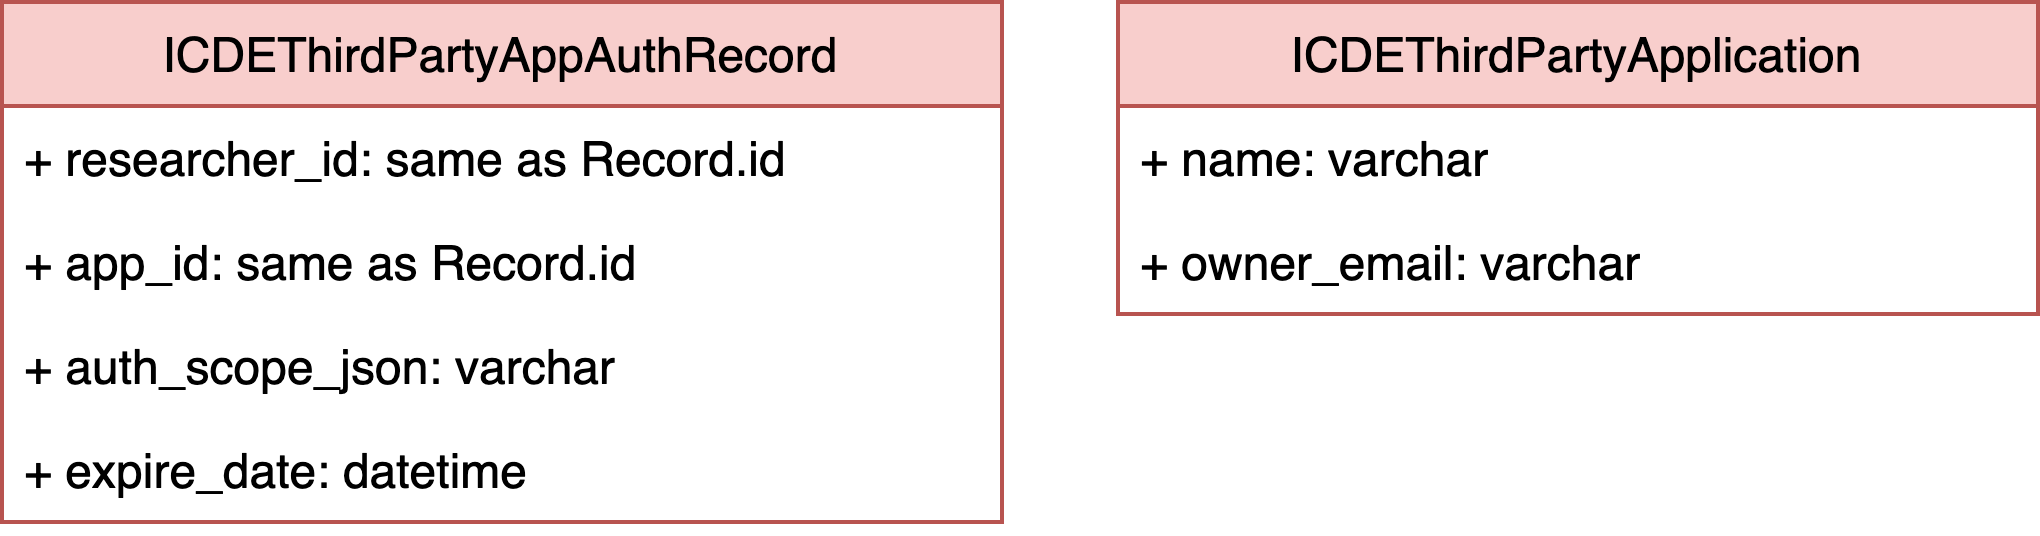
\includegraphics[width=0.75\textwidth]{./img/bo_classes_6.png}
	\caption{Bussiness Objects Part5: ICDEThirdPartyApplication, ICDEThirdPartyAppAuthRecord}
	
	\label{fig:bo_classes_6}
\end{figure*}

\textbf{Representative Diagrem for Key SRS}

For SRS1.1.1-Register, it can be represent as activity diagram shown in Fig. \ref{fig:srs_diagram_1}.

\begin{figure*}[t]
	\centering
	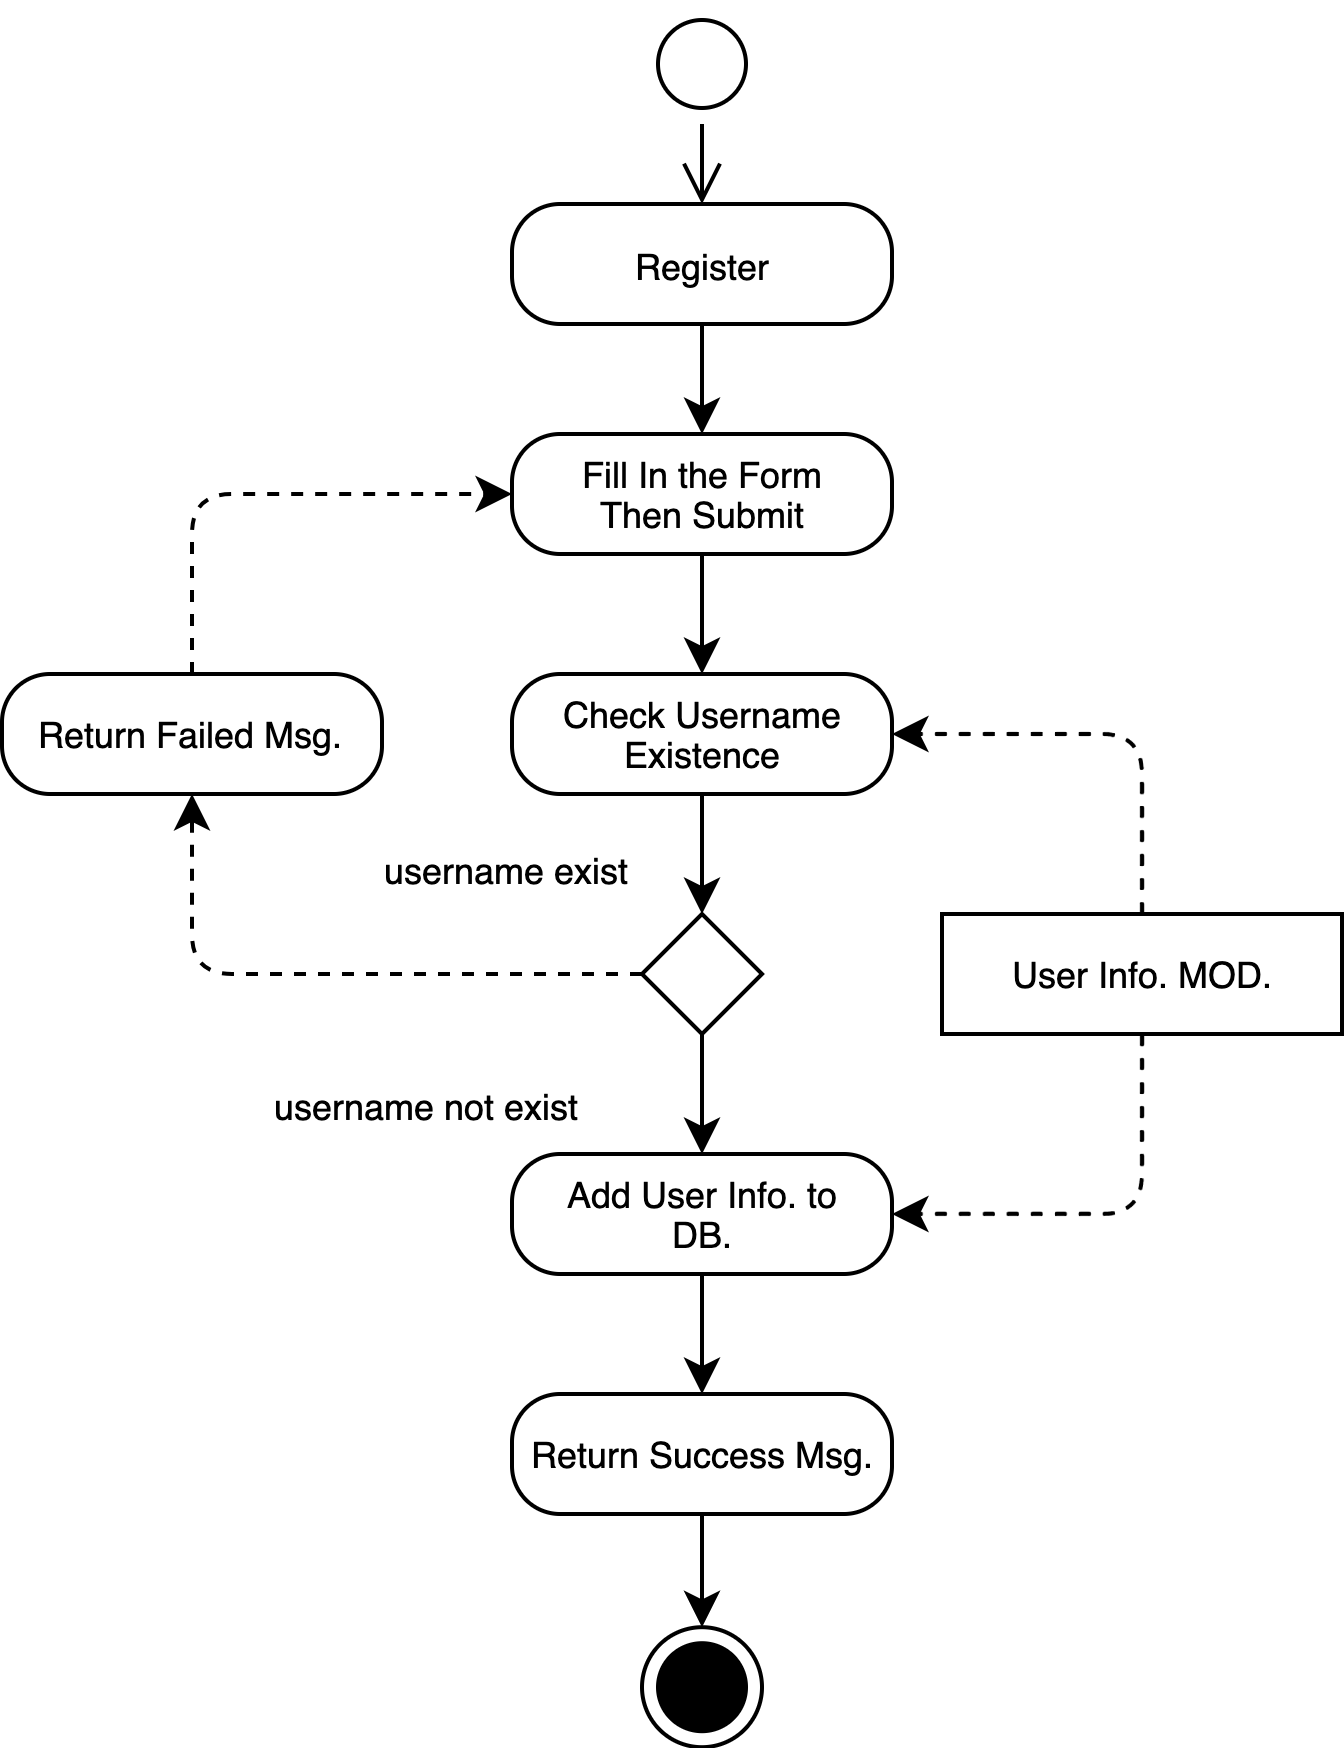
\includegraphics[width=0.6\textwidth]{./img/srs_diagram_1.png}
	\caption{Activity Diagram for SRS1.1.1}
	
	\label{fig:srs_diagram_1}
\end{figure*}

For SRS1.1.2-Update User informations, it can be represent as activity diagram shown in Fig. \ref{fig:srs_diagram_2}.

\begin{figure*}[t]
	\centering
	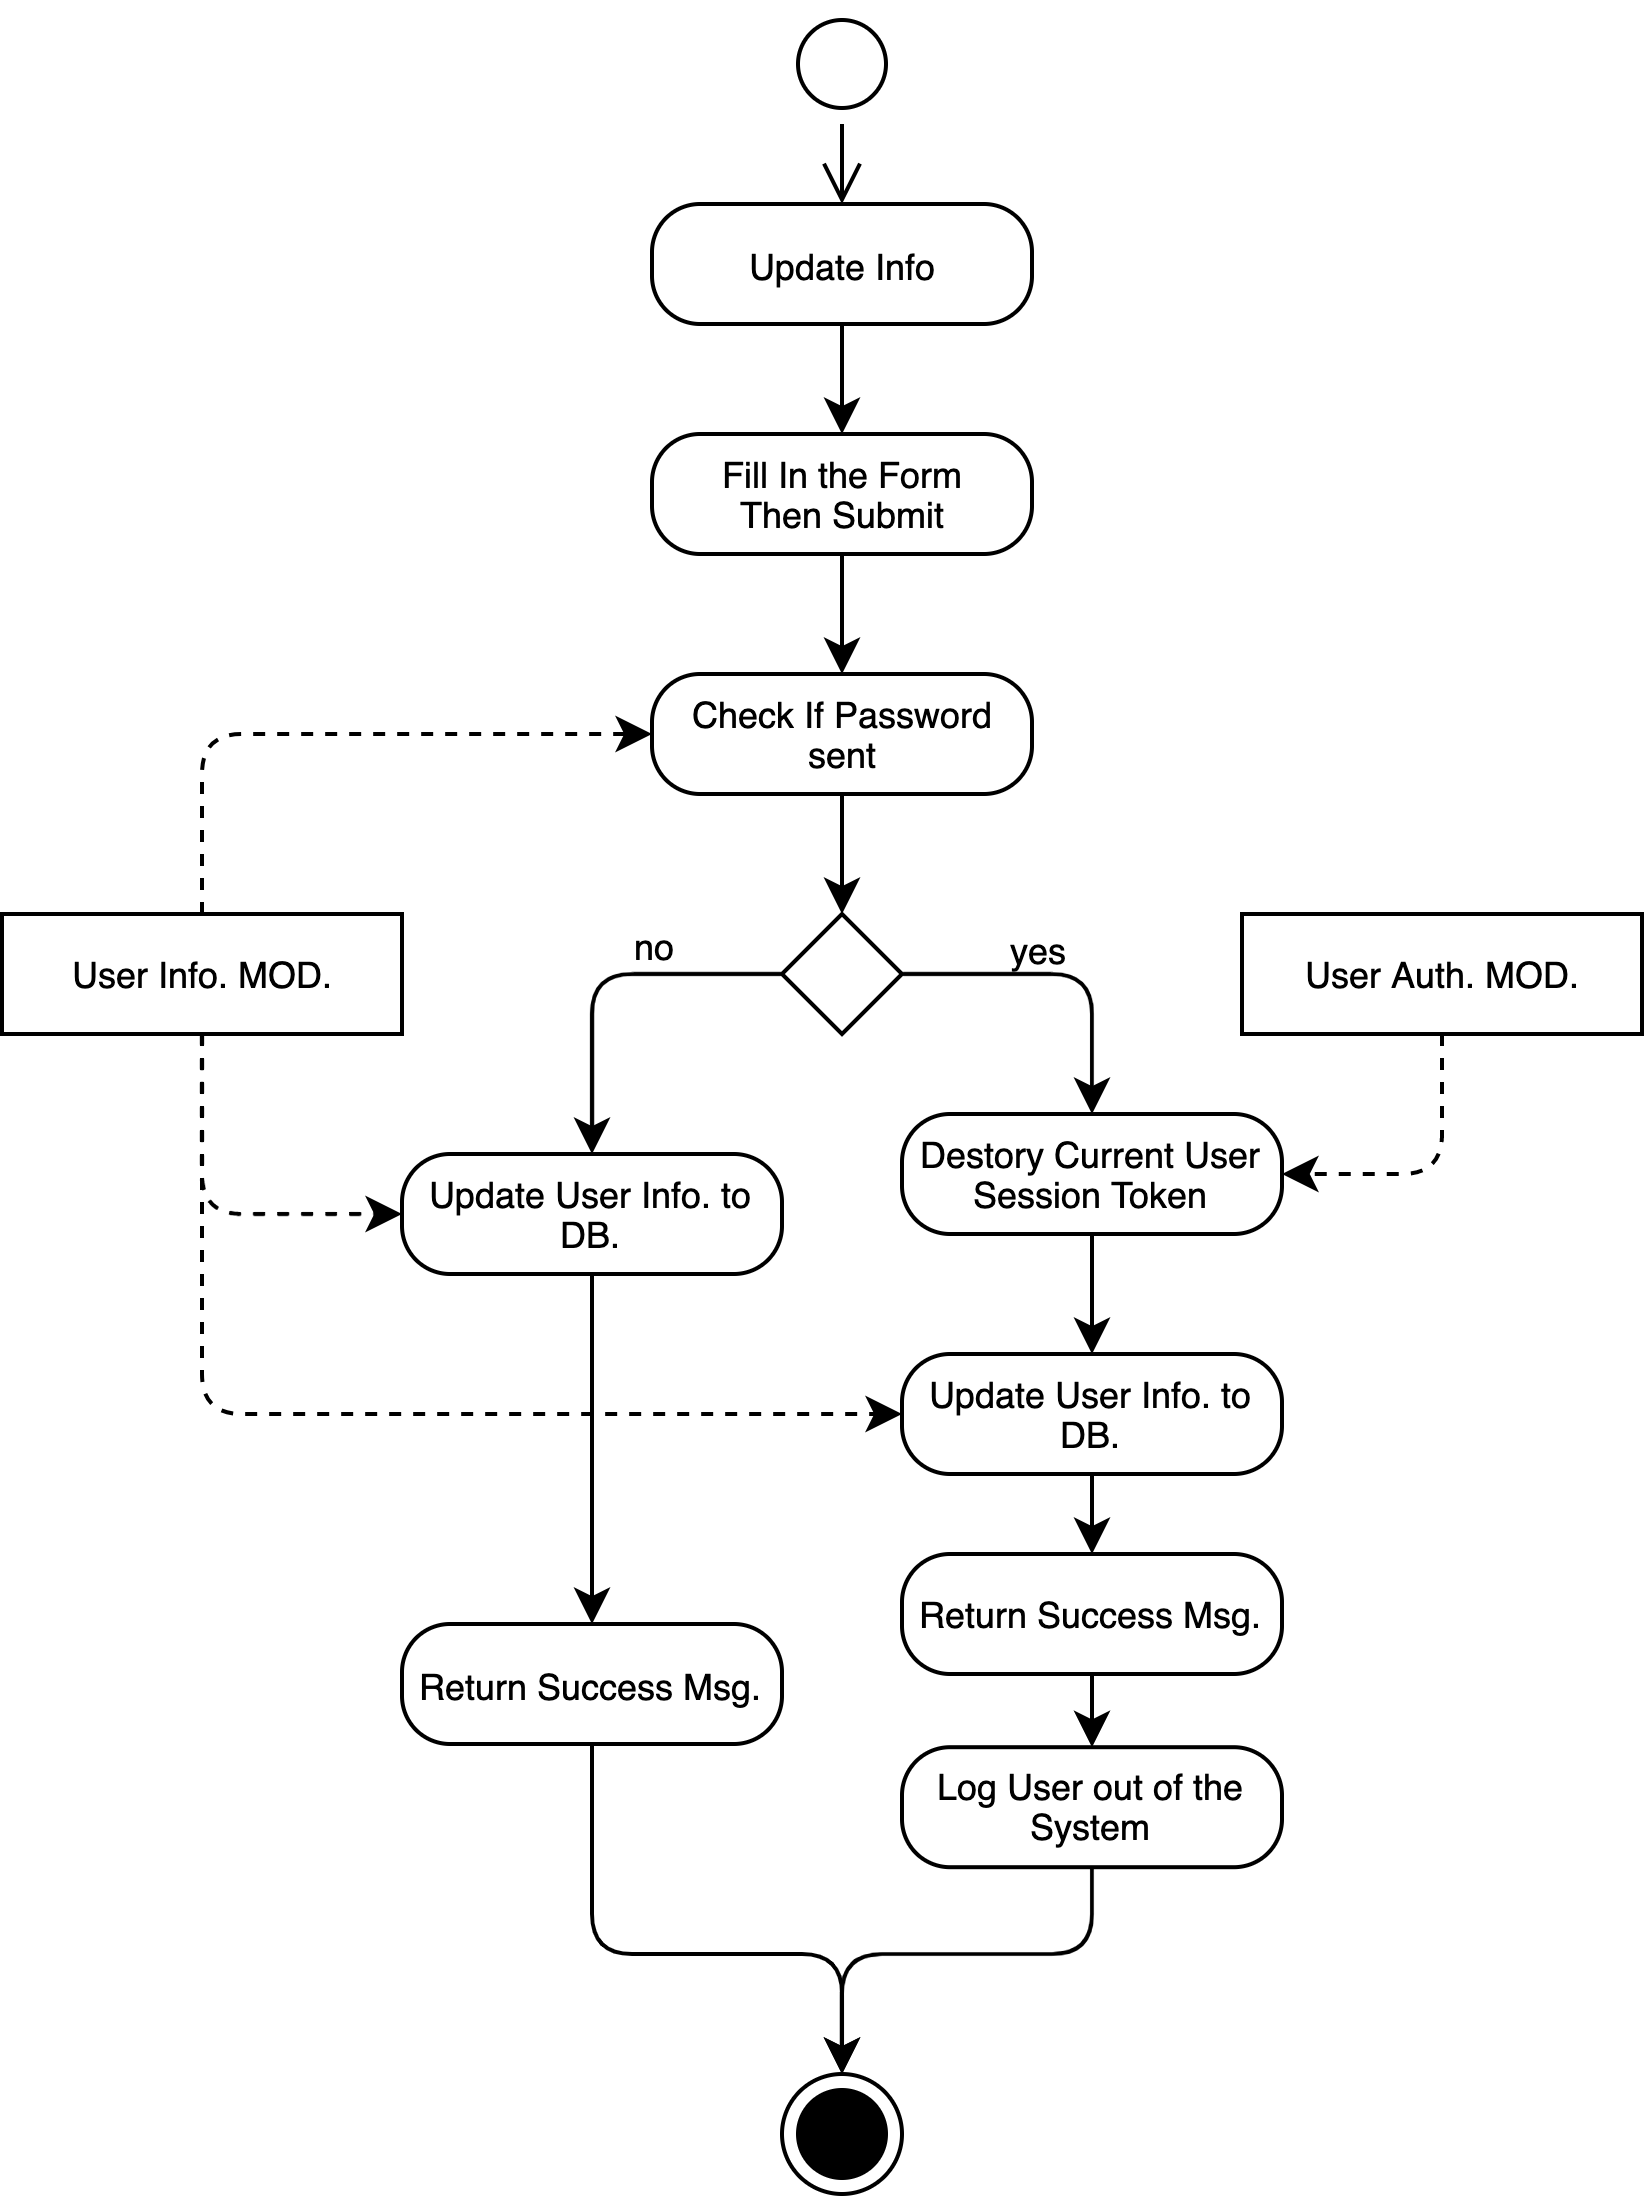
\includegraphics[width=0.6\textwidth]{./img/srs_diagram_2.png}
	\caption{Activity Diagram for SRS1.1.2}
	\label{fig:srs_diagram_2}
\end{figure*}

For SRS1.2.1-Login, it can be represent as activity diagram shown in Fig. \ref{fig:srs_diagram_3}.

\begin{figure*}[t]
	\centering
	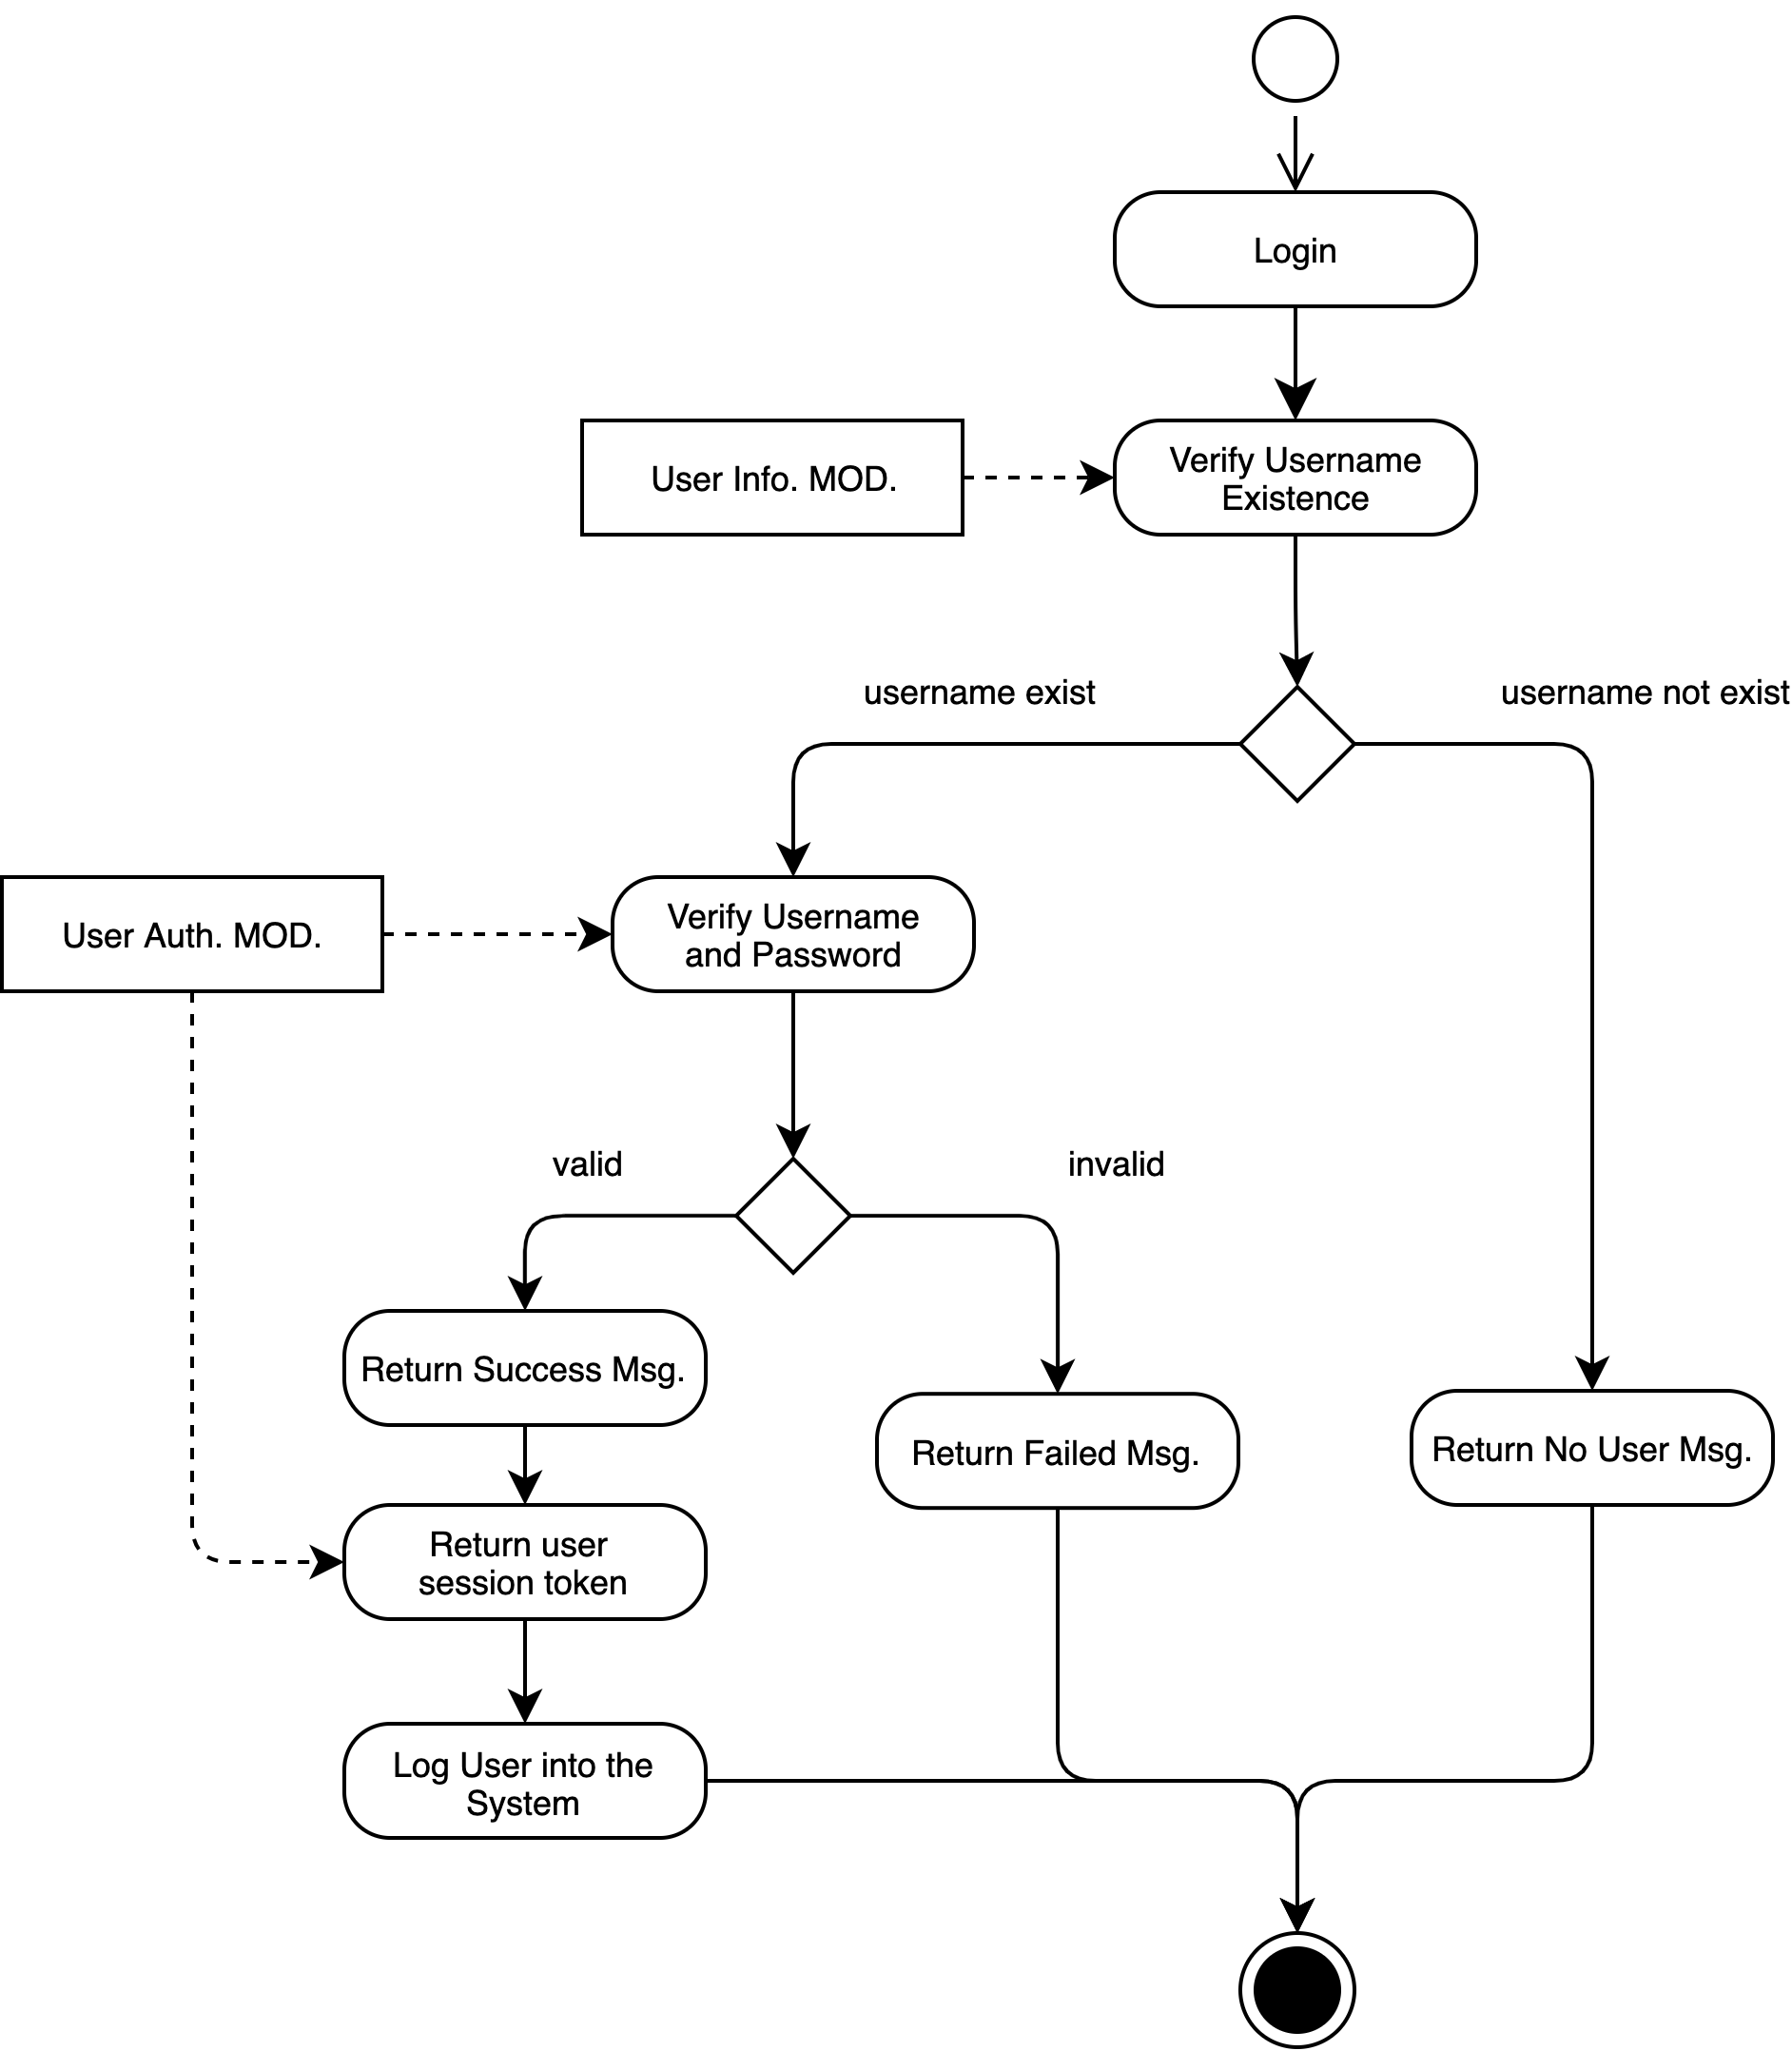
\includegraphics[width=0.6\textwidth]{./img/srs_diagram_3.png}
	\caption{Activity Diagram for SRS1.2.1}
	
	\label{fig:srs_diagram_3}
\end{figure*}


For SRS2.1.1-Download Paper, it can be represent as sequence diagram shown in Fig. \ref{fig:srs_diagram_4}.

\begin{figure*}[t]
	\centering
	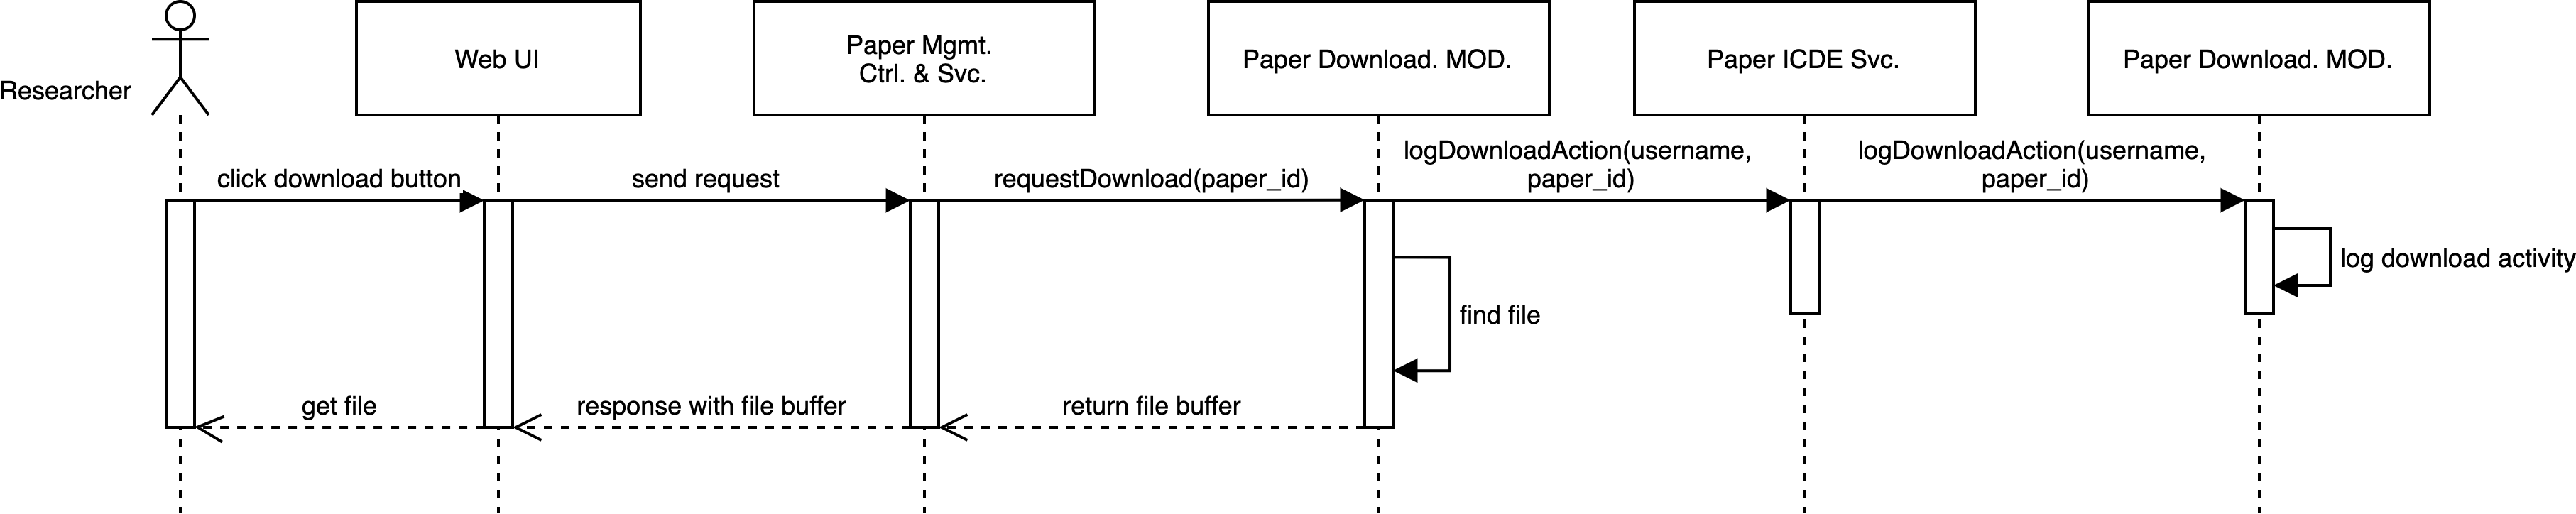
\includegraphics[width=1\textwidth]{./img/srs_diagram_4.png}
	\caption{Sequence Diagram for SRS2.1.1}
	
	\label{fig:srs_diagram_4}
\end{figure*}


For SRS 2.1.2, SRS 2.2.4, SRS 4.2, and SRS 5, they can be represent as activity diagram shown in Fig. \ref{fig:srs_diagram_5}.

\begin{figure*}[t]
	\centering
	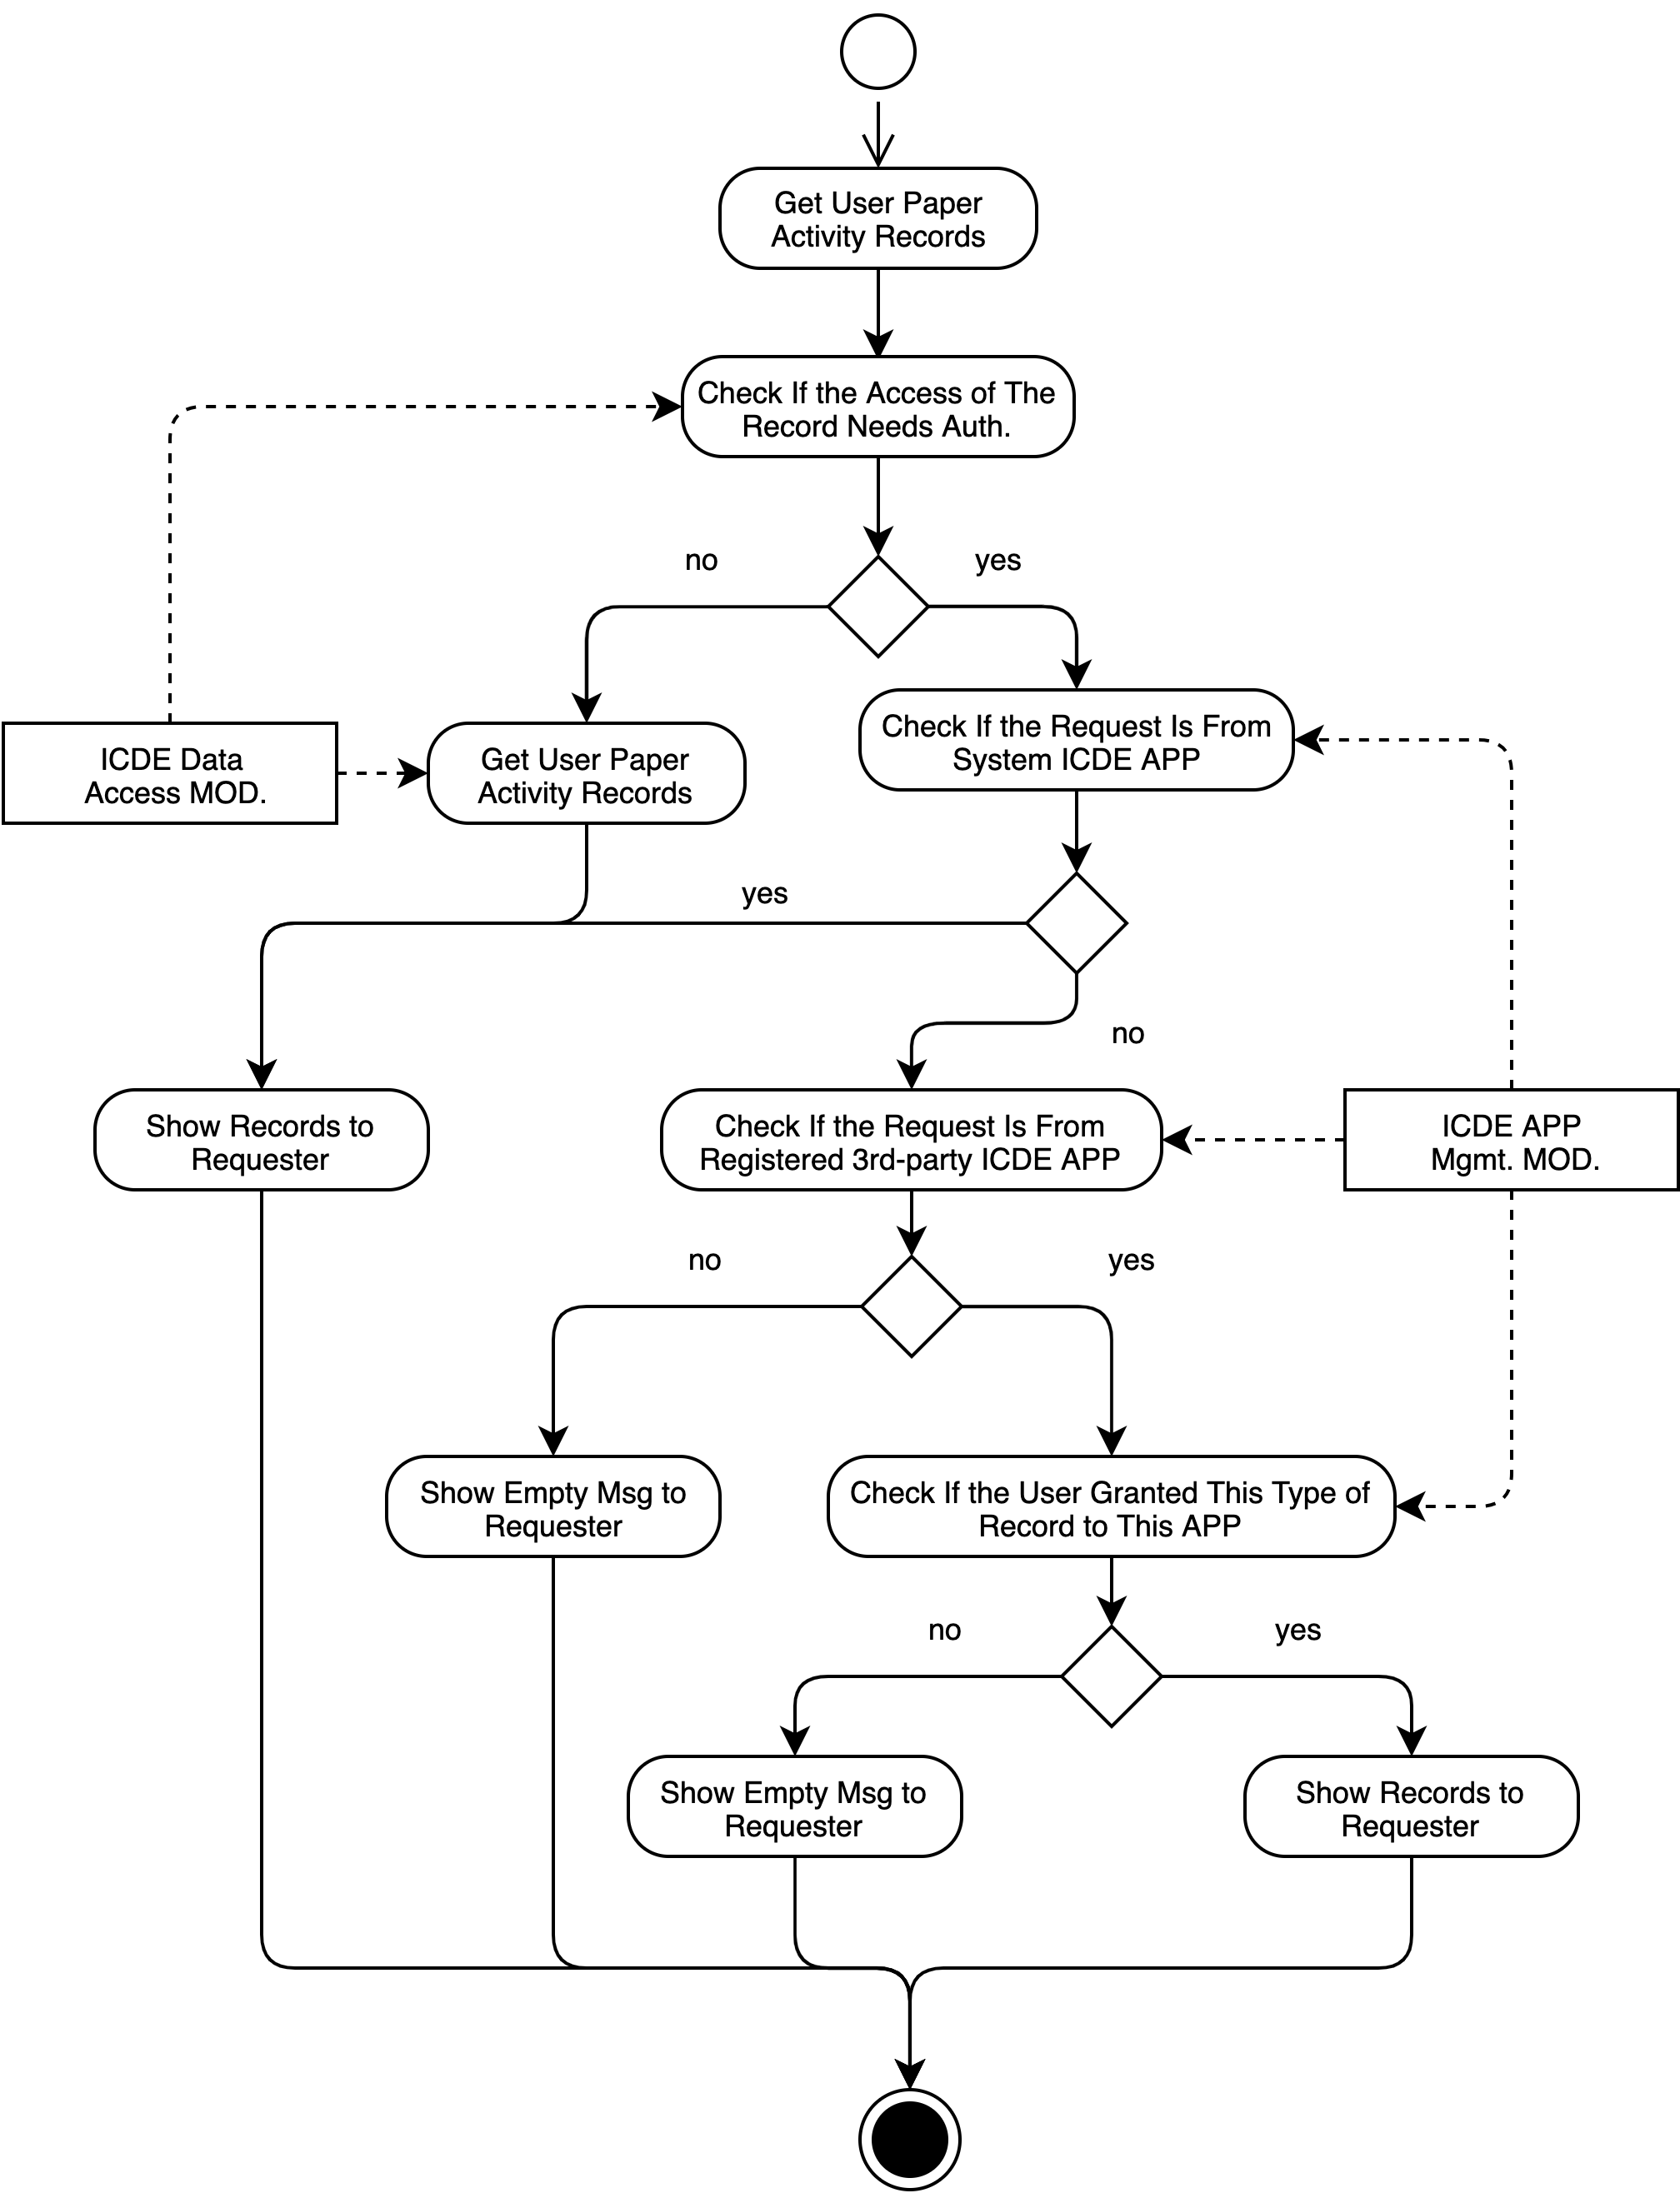
\includegraphics[width=0.6\textwidth]{./img/srs_diagram_5.png}
	\caption{Activity Diagram for SRS 2.1.2, SRS 2.2.4, SRS 4.2, and SRS 5}
	
	\label{fig:srs_diagram_5}
\end{figure*}

For SRS 6.1.2-Team Invitation, it can be represent as activity diagram shown in Fig. \ref{fig:srs_diagram_6}. 
Also it indicates how ICDE functions. And its sequence diagram is shown in Fig. \ref{fig:srs_diagram_7}. 
And also its state diagram shown in Fig. \ref{fig:srs_diagram_8}

\begin{figure*}[t]
	\centering
	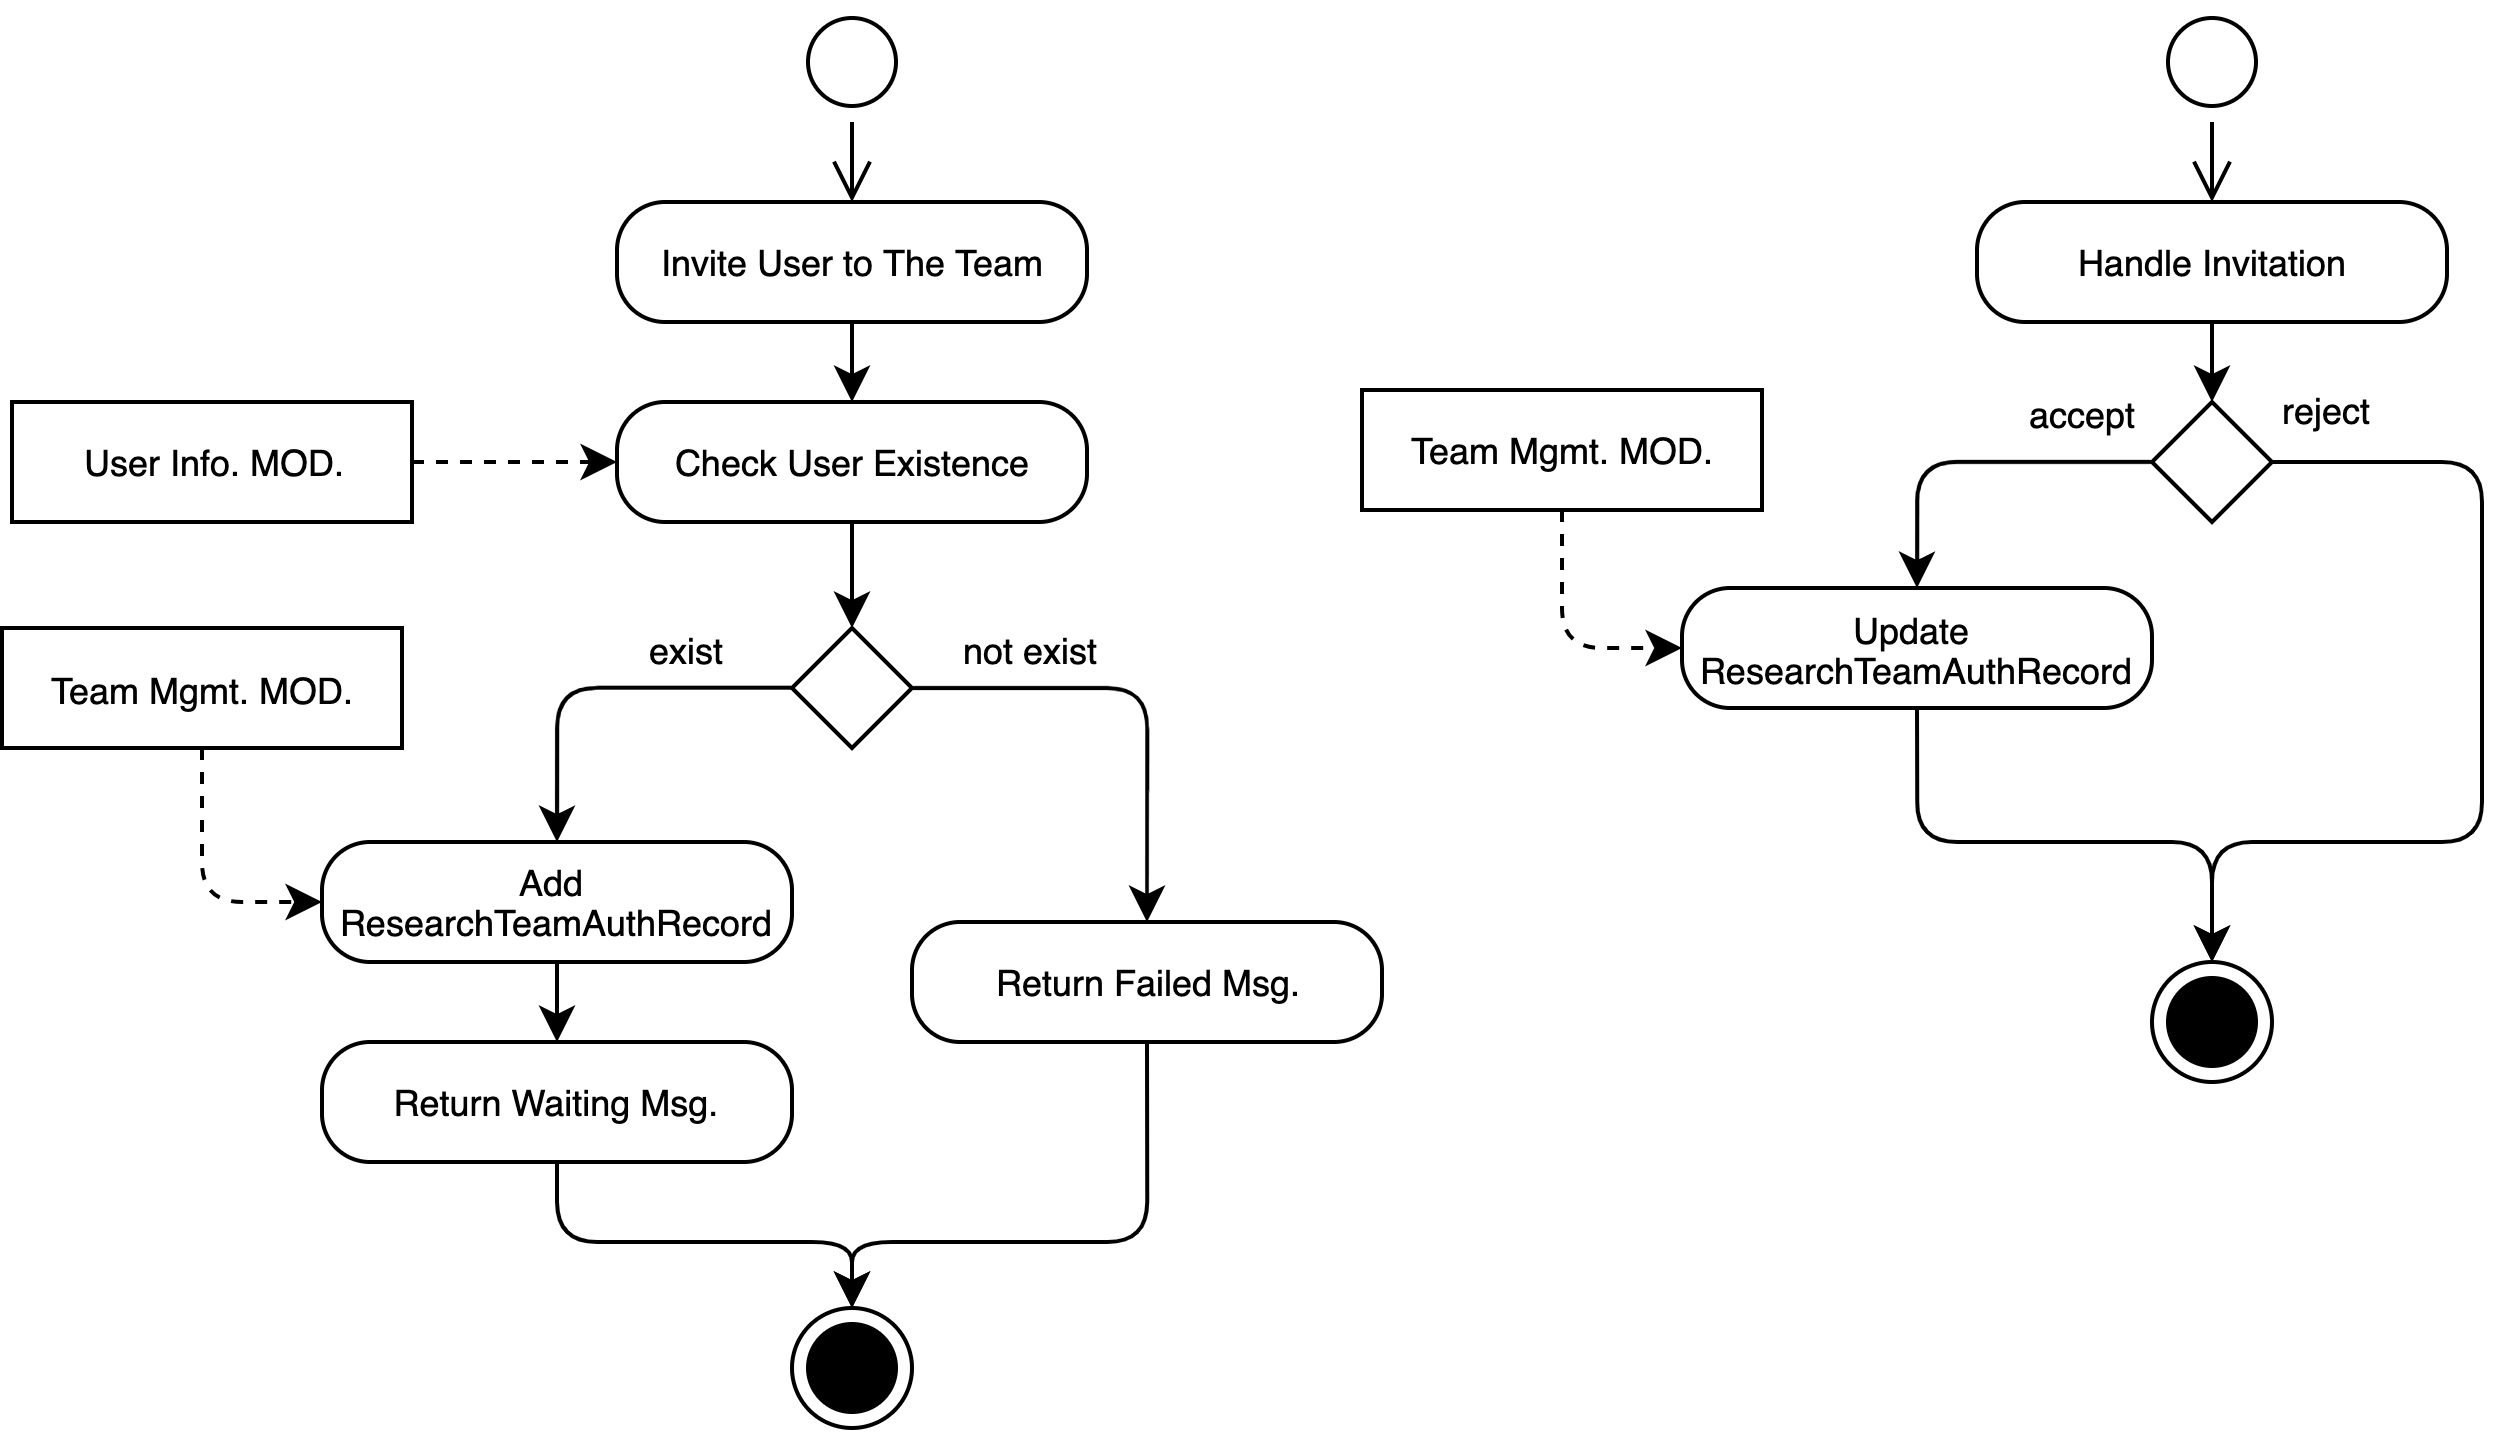
\includegraphics[width=0.8\textwidth]{./img/srs_diagram_6.png}
	\caption{Activity Diagram for SRS 6.1.2}
	
	\label{fig:srs_diagram_6}
\end{figure*}

\begin{figure*}[t]
	\centering
	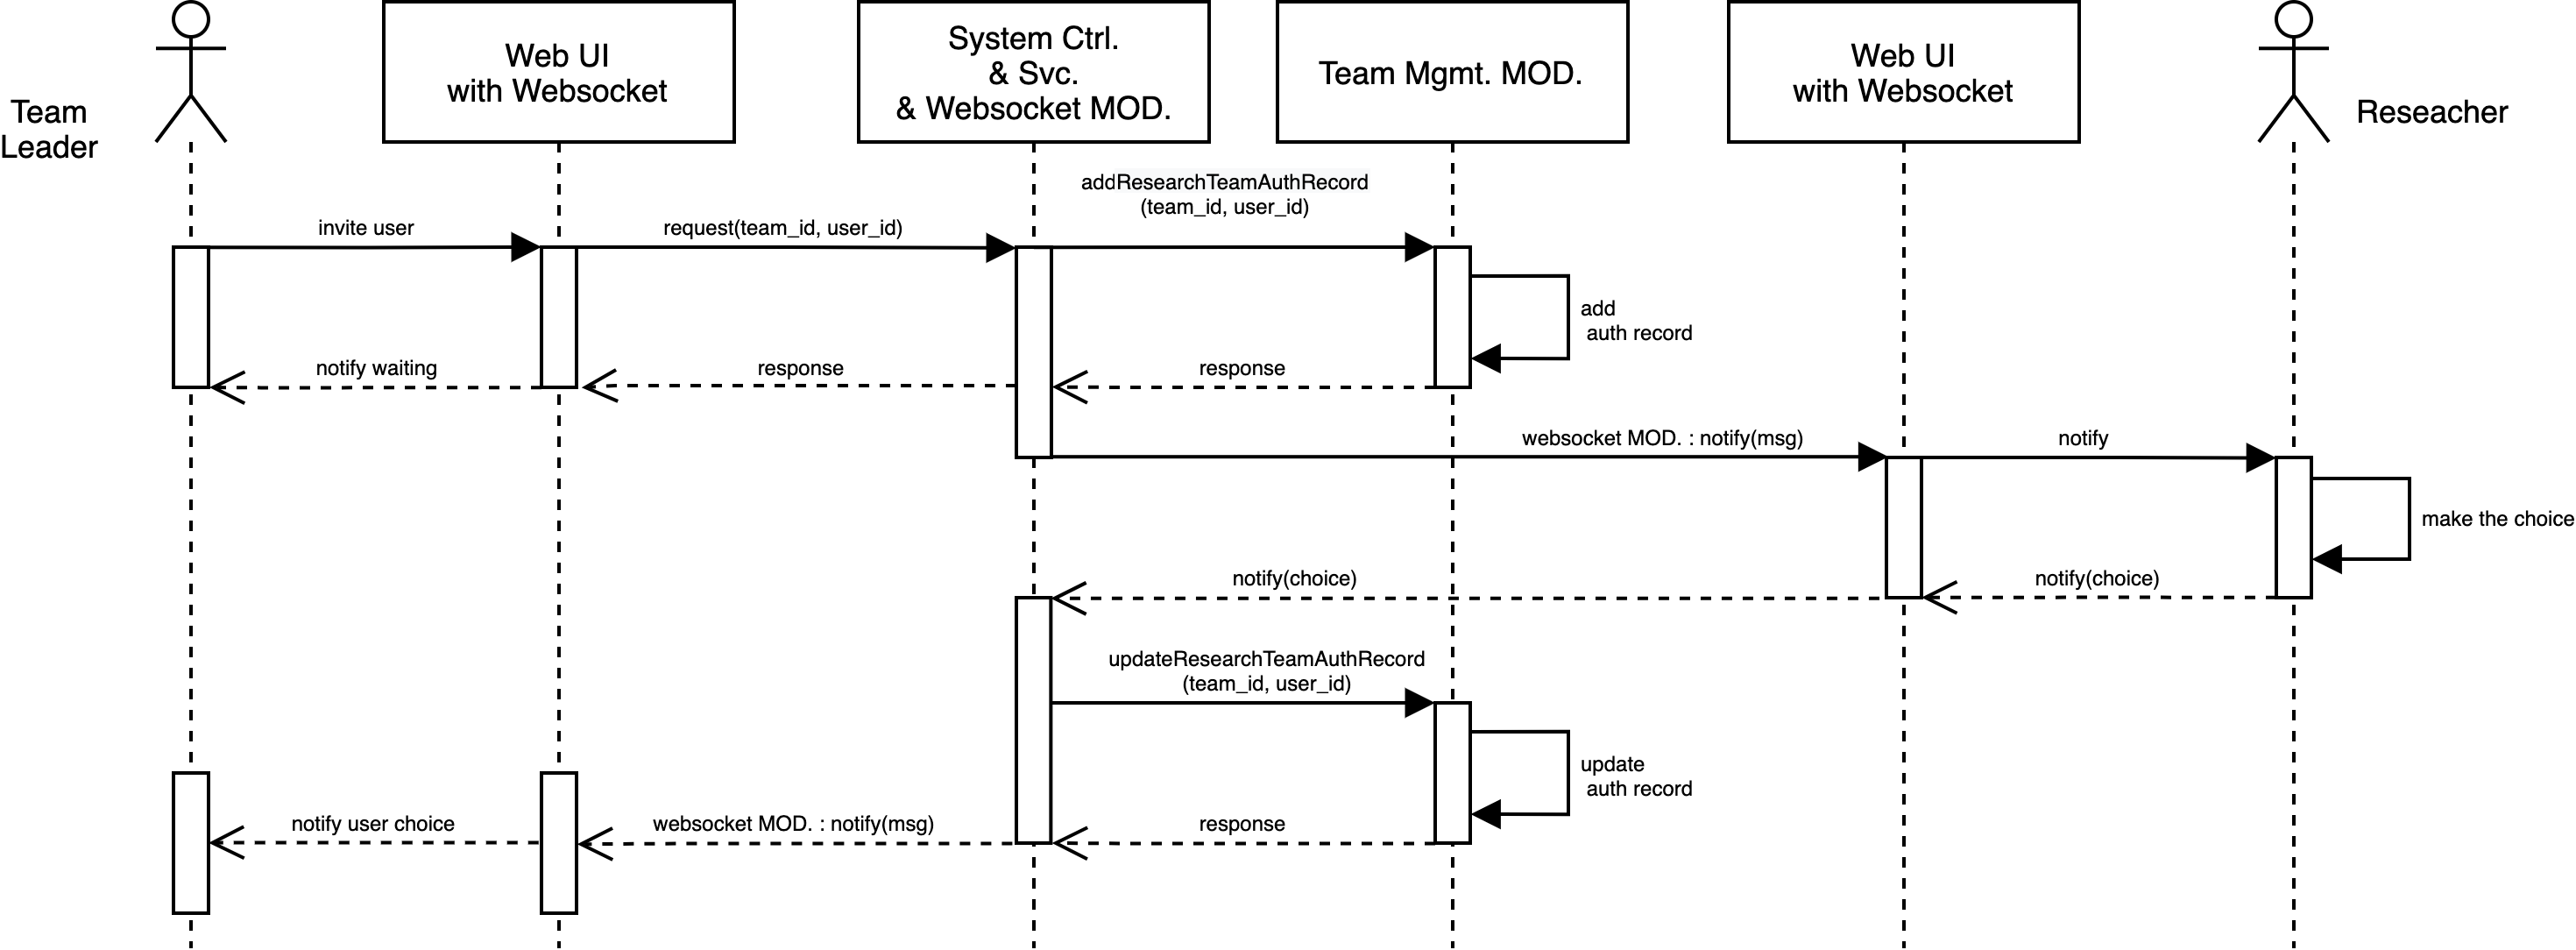
\includegraphics[width=\textwidth]{./img/srs_diagram_7.png}
	\caption{Sequence Diagram for SRS 6.1.2}
	
	\label{fig:srs_diagram_7}
\end{figure*}

\begin{figure*}[t]
	\centering
	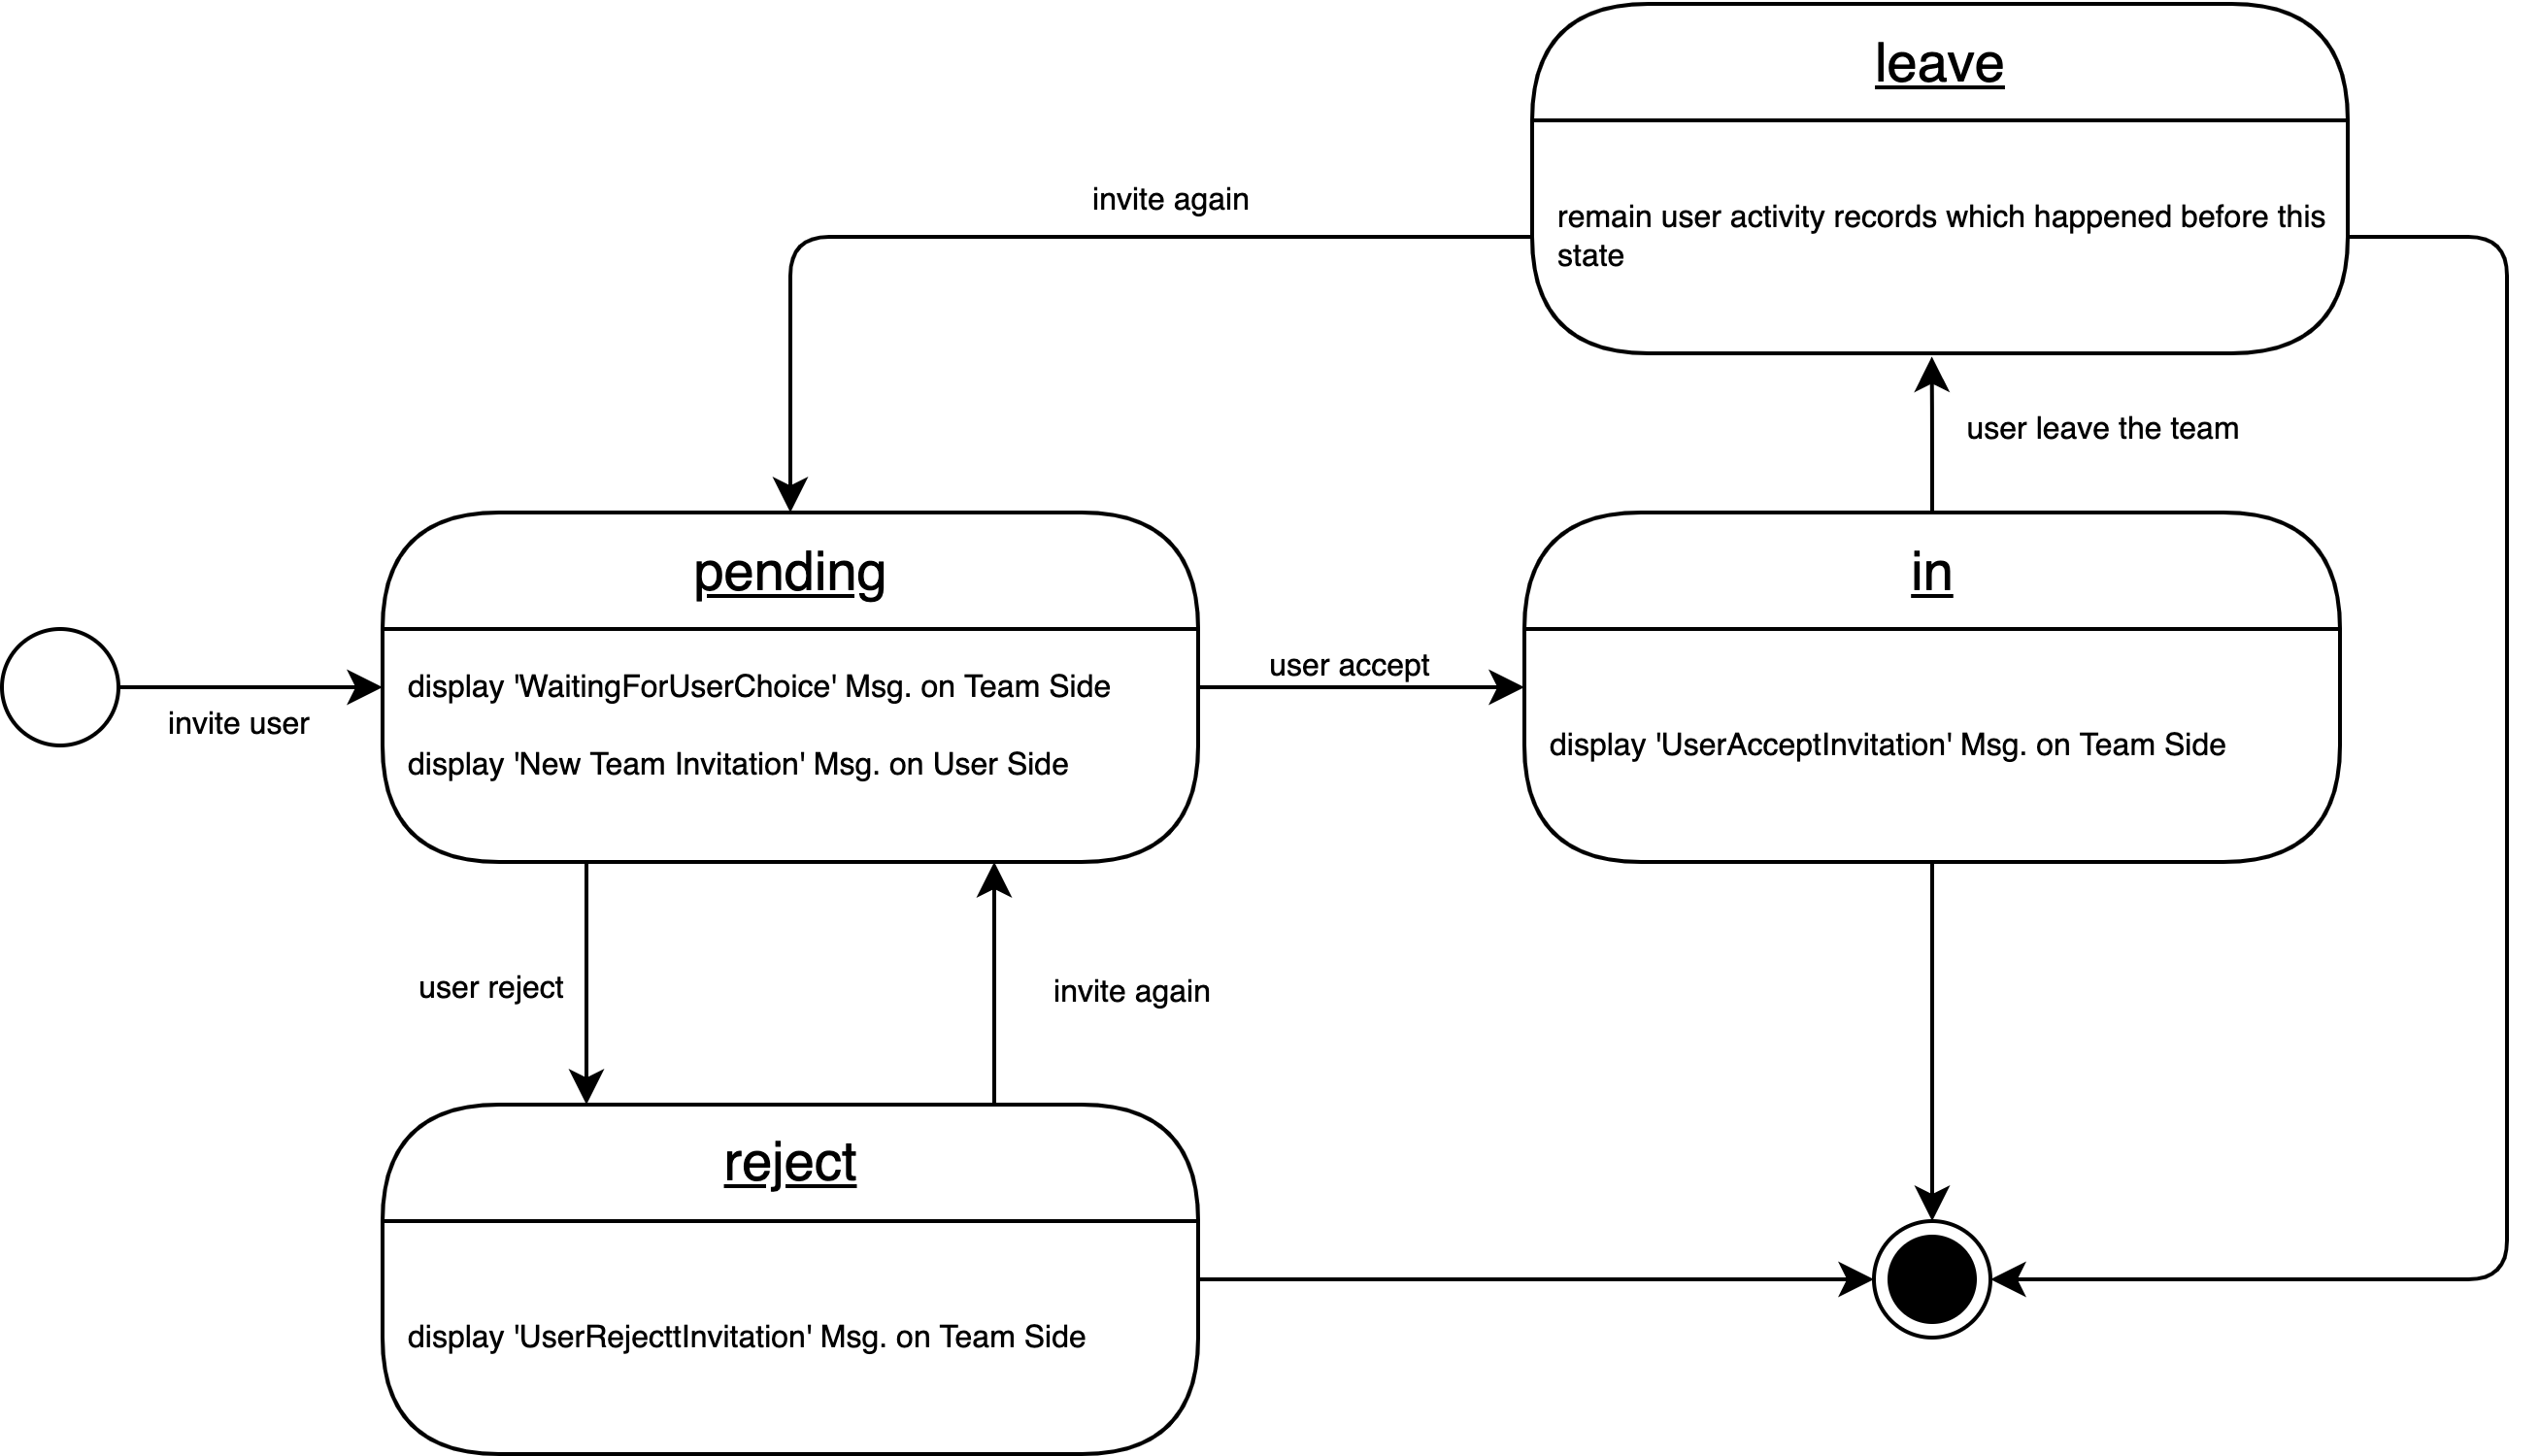
\includegraphics[width=0.8\textwidth]{./img/srs_diagram_8.png}
	\caption{State Diagram for SRS 6.1.2}
	
	\label{fig:srs_diagram_8}
\end{figure*}
